\newpage
\section*{Technologierecherche}
Zu Beginn der Recherchephase wurde der Roboter anhand der Anforderungsliste in einzelne Teilfunktionen zerlegt. Somit konnte der Vorgang der Recherche besser paralleilisert werden und es ist eifacher die Übersicht zu behalten (Divide et impera). Die folgenden Teilfunktionen tauchen in der gesamten Dokumentation immer wieder auf:
\begin{itemize}
    \item Fortbewegung
    \item Lenkung
    \item Treppensteigen
    \item Orientierung
    \item Bilderkennung
    \item Auftragsquittierung
    \item Antrieb
    \item Not-Aus
    \item Energiequelle
    \item Steuerung
\end{itemize}
\subsection*{Überblick}
Nachfolgend ist ein kurzer Überblick über die Technologierecherche in Tabellenform (siehe Tabelle \ref{tab:technologierecherche}). Für die detaillierte Technologierecherche siehe Anhang: Abschnitt Detailrecherche.

\scriptsize
\begin{longtable}{l@{\extracolsep{\fill}}p{2cm}p{2cm}p{4cm}p{3cm}lll}
%\toprule
\textbf{Dep.} & \textbf{Teilfunktion} & \textbf{Thema} &
\textbf{Beschreibung} & \textbf{Quelle} & \textbf{Abfragedatum} &
\textbf{Wer}\tabularnewline
%\midrule
\endhead

M
 & 
Fortbewegung
 & 
Motorik
 & 
PowerPoint

Fortbewegung Robotik
 & 
\tiny\url{https://www.informatik.uni-bremen.de/~roefer/kr00/03.pdf}
 & 
 25.09.2020
 & 
Sven
\tabularnewline

M
 & 
Fortbewegung
 & 
Normale Räder
 & 
YouTube Video

Rasenmähroboter mit Allradantrieb
 & 
\tiny\url{https://www.youtube.com/watch?v=nln_zyRJHqQ}
 & 
25.09.2020
 & 
Sven
\tabularnewline

M
 & 
Lenkung
 & 
Lenkachse
 & 
Wikipedia Artikel

Ackermann-Lenkung
 & 
\tiny\url{https://de.wikipedia.org/wiki/Lenkung}
 & 
27.09.2020
 & 
Sven
\tabularnewline

M
 & 
Lenkung
 & 
Lenkachse
 & 
YouTube Video

Legofahrzeug mit Lenkachse
 & 
\tiny\url{https://www.youtube.com/watch?v=Y47LjdiEOuY}
 & 
27.09.2020
 & 
Sven
\tabularnewline

M
 & 
Lenkung
 & 
Knicklenkung
 & 
Wikipedia Artikel

Knicklenkung
 & 
\tiny\url{https://de.wikipedia.org/wiki/Knicklenkung}
 & 
27.09.2020
 & 
Sven
\tabularnewline

M
 & 
Lenkung
 & 
Panzerlenkung
 & 
Wikipedia Artikel

Knicklenkung
 & 
\tiny\url{https://www.rs-online.com/designspark/give-your-robot-the-mobility-control-of-a-real-mars-rover-part-4-de}
 & 
27.09.2020
 & 
Sven
\tabularnewline

M
 & 
Lenkung
 & 
Roomba-Lenkprinzip
 & 
YouTube Video

Roomba Staubsaugroboter
 & 
\tiny\url{https://www.youtube.com/watch?v=J6rMaLYq5cA}
 & 
27.09.2020
 & 
Sven
\tabularnewline

M
 & 
Fortbewegung
 & 
Omnidrive-Allseitenräder
 & 
Wikipedia Artikel

Omnidrive
 & 
\tiny\url{https://de.wikipedia.org/wiki/Omnidirektionaler_Antrieb}
 & 
25.09.2020
 & 
Sven
\tabularnewline

M
 & 
Fortbewegung
 & 
Omnidrive-Allseitenräder
 & 
YouTube Video

Fahrzeug mit 3 Allseitenräder
 & 
\tiny\url{https://www.youtube.com/watch?v=hCVpIUzlsl8}
 & 
25.09.2020
 & 
Sven
\tabularnewline

M
 & 
Fortbewegung
 & 
Omnidrive-Mecanumräder
 & 
Wikipedia Artikel

Mecanumrad
 & 
\tiny\url{https://de.wikipedia.org/wiki/Mecanum-Rad}
 & 
25.09.2020
 & 
Sven
\tabularnewline

M
 & 
Fortbewegung
 & 
Omnidrive-Mecanumräder
 & 
YouTube Video

Fahrzeug mit 4 Mecanumräder
 & 
\tiny\url{https://www.youtube.com/watch?v=Ne09Y72zW_Y}
 & 
27.09.2020
 & 
Sven
\tabularnewline

M
 & 
Fortbewegung
 & 
Omnidrive-Fahrdrehmodul
 & 
YouTube Video

Legoroboter mit Fahrdrehmodul
 & 
\tiny\url{https://www.youtube.com/watch?v=wGLnRLmW3A8}
 & 
27.09.2020
 & 
Sven
\tabularnewline

M
 & 
Fortbewegung
 & 
Omnidrive-Fahrdrehmodul
 & 
Wikipedia Artikel

Fahrdrehmodul
 & 
\tiny\url{https://de.wikipedia.org/wiki/Omnidirektionaler_Antrieb\#Allseitenr\%C3\%A4der}
 & 
27.09.2020
 & 
Sven
\tabularnewline

M
 & 
Fortbewegung
 & 
Verschiedene

Räderarten
 & 
Gegenüberstellung Räderarten
 & 
\tiny\url{https://silo.tips/download/fahrwerkskonzept-gegenberstellung}
 & 
25.09.2020
 & 
Sven
\tabularnewline

M
 & 
Fortbewegung
 & 
Propeller
 & 
Wissensartikel

Wie funktioniert eine Drohne
 & 
\tiny\url{https://u-rob.com/wissensartikel/wie-funktioniert-eine-drohne/}
 & 
25.09.2020
 & 
Sven
\tabularnewline

M
 & 
Fortbewegung
 & 
Propeller
 & 
Wikipedia Artikel

Quadrokopter
 & 
\tiny\url{https://de.wikipedia.org/wiki/Quadrocopter}
 & 
25.09.2020
 & 
Sven
\tabularnewline

M
 & 
Fortbewegung
 & 
Beine
 & 
YouTube Video

Roboter mit 4 Beinen
 & 
\tiny\url{https://www.youtube.com/watch?v=M8YjvHYbZ9w}
 & 
27.09.2020
 & 
Sven
\tabularnewline

M
 & 
Fortbewegung
 & 
Beine
 & 
Wissensartikel

Wie Roboter Laufen lernen
 & 
\tiny\url{https://www.it-zoom.de/mobile-business/e/wie-die-roboter-laufen-lernen-22299/}
 & 
27.09.2020
 & 
Sven
\tabularnewline

M
 & 
Fortbewegung
 & 
Beine
 & 
Wikipedia Artikel

Laufroboter
 & 
\tiny\url{https://de.wikipedia.org/wiki/Laufroboter}
 & 
27.09.2020
 & 
Sven
\tabularnewline
M & Treppensteigen & Spezielle Treppenräder & Bau eines
Treppensteigroboters &
\tiny\url{https://www.instructables.com/id/Stair-Climbing-Robot-1/}
& 27.09.2020 & Sven\tabularnewline

M
 & 
Treppensteigen
 & 
Hebemechanismus: 3-Teilig
 & 
YouTube Video

ZHAW Projekt
 & 
\tiny\url{https://www.youtube.com/watch?v=zRefD--ESzw}
 & 
23.09.2020
 & 
Sven
\tabularnewline
M & Treppensteigen & Hebemechanismus: Raufklappen  & 
YouTube Video

ZHAW Projekt
 & 
\tiny\url{https://www.youtube.com/watch?v=zRefD--ESzw}
 & 
23.09.2020
 & 
Sven\tabularnewline
M & Treppensteigen & Hebemechanismus: Aufstapeln und Ausfahren  & 
YouTube Video

ZHAW Projekt
 & 
\tiny\url{https://www.youtube.com/watch?v=zRefD--ESzw}
 & 
23.09.2020
 & 
Sven\tabularnewline
M & Treppensteigen & Hebemechanismus: 3-Teilig & YouTube Video &
\tiny\url{https://www.youtube.com/watch?v=MWkYDJd66to}
& 27.09.2020 & Sven\tabularnewline
M & Treppensteigen & Hebemechanismus: Raufklappen & YouTube Video &
\tiny\url{https://www.youtube.com/watch?v=8DSh4Y_wyKQ}
& 27.09.2020 & Sven\tabularnewline
M & Treppensteigen & Hebemechanismus: Aufstapeln und Ausfahren & YouTube
Video &
\tiny\url{https://www.youtube.com/watch?v=TQCqQGbE2Sk}
& 27.09.2020 & Sven\tabularnewline

M
 & 
Treppensteigen
 & 
Katapult
 & 
YouTube Video

Legokatapultroboter
 & 
\tiny\url{https://www.youtube.com/watch?v=rcgC4nv1jNE}
 & 
27.09.2020
 & 
Sven
\tabularnewline

M
 & 
Treppensteigen
 & 
Sprungfeder
 & 
Wissensartikel

Sprung Roboter
 & 
\tiny\url{https://www.ingenieur.de/technik/fachbereiche/robotik/roboter-affe-salto-gewaltige-spruenge/}
 & 
27.09.2020
 & 
Sven
\tabularnewline

M
 & 
Treppensteigen
 & 
Sprungfeder
 & 
YouTube Video

Roboter der springen kann
 & 
\tiny\url{https://www.youtube.com/watch?v=pMRwU6ugSvs}
 & 
27.09.2020
 & 
Sven
\tabularnewline

M
 & 
Treppensteigen
 & 
Bahn ausfahren für kleines Fahrzeug
 & 
YouTube Video

Lego Technik Bridge Girder
 & 
\tiny\url{https://www.youtube.com/watch?v=Ny-ighFGg98}
 & 
27.09.2020
 & 
Sven
\tabularnewline

M
 & 
Treppensteigen
 & 
Schlange mit Magneten
 & 
YouTube Video

Schlangenroboter besteigt Treppe
 & 
\tiny\url{https://www.youtube.com/watch?v=GROAOduaH0A}
 & 
27.09.2020
 & 
Sven
\tabularnewline
I & Orientierung & Tastsensor & Roboter erkennt Hindernisse durch einen
Tastsensor &
\tiny\url{https://rn-wissen.de/wiki/index.php/Tastsensoren}~
& 05.10.2020 & Yves\tabularnewline

I
 & 
Orientierung
 & 
Distanzsensor
 & 
Roboter erkennt Hindernisse und kann Distanzen mithilfe von
Distanzsensoren messen z.B. mittels Radar oder Ultraschall
 & 
\tiny\url{https://www.mikrocontroller-elektronik.de/ultraschallsensor-hc-sr04/}~

\tiny\url{https://agilsense.com/product/detail/3}~
 & 
05.10.2020
 & 
Yves
\tabularnewline
I & Orientierung & Kamera & Roboter erkennt Hindernisse durch eine
Kamera & \tiny\url{https://www.pi-shop.ch/raspberry-pi-kamera-module-v2}~ &
05.10.2020 & Yves\tabularnewline
I & Orientierung & GPS & Roboter kann sich mithilfe seines eigenen
Standortes orientieren &
\tiny\url{https://www.netzwelt.de/gps/index.html\#funktioniert-gps}~
& 05.10.2020 & Yves\tabularnewline

I
 & 
Orientierung
 & 
Lidar (Light detection and ranging)
 & 
Distanzmessung durch Bestrahlung mit Laser und messen der Zeit bis die
Strahlen reflektiert werden
 & 
\tiny\url{https://www.laserscanning-europe.com/de/glossar/funktionsweise-eines-laserscanners}

\tiny\url{https://www.pi-shop.ch/lidar-lite-v3}
 & 
05.10.2020
 & 
Yves
\tabularnewline

I
 & 
Orientierung
 & 
Beschleunigungssensor
 & 
Der Beschleunigungssensor misst beschleunigende Kräfte, sowohl statische
wie die Gravitation, als auch dynamische wie Rütteln oder Kippen.
 & 
\tiny\url{https://rn-wissen.de/wiki/index.php?title=Sensoren_-_Beschleunigung}~

\tiny\url{https://www.dimensionengineering.com/info/accelerometers}
 & 
05.10.2020
 & 
Yves
\tabularnewline

I
 & 
Orientierung
 & 
TOF-Sensor
 & 
Mit einem TOF-Sensor kann man Tiefeninformationen sammeln, um
Strukturen, Entfernungen von Gegenständen, und Bewegungen genau zu
ermitteln
 & 
\tiny\url{https://www.st.com/en/imaging-and-photonics-solutions/proximity-sensors.html}

\tiny\url{https://www.giga.de/artikel/tof-sensor-time-of-flight-was-ist-das-wofuer-wird-er-verwendet/}
 & 
05.10.2020
 & 
Yves
\tabularnewline

I
 & 
Bilderkennung
 & 
Google Vision API
 & 
Die Vision API von Google Cloud bietet über die REST API und die RPC API
vorab trainierte Modelle für maschinelles Lernen. Damit kann man Bildern
Labels zuweisen und die Bilder Millionen vordefinierter Kategorien
zuweisen.
 & 
Übersicht:
\tiny\url{https://cloud.google.com/vision/\#industry-leading-accuracy-for-image-understanding}

API Reference: \tiny\url{https://cloud.google.com/vision/docs/reference/rest}

Preis: \tiny\url{https://cloud.google.com/vision/pricing}
 & 
25.09.2020
 & 
Boas
\tabularnewline
I & Bilderkennung & CognitiveJ & CognitiveJ ist eine Open-Source Java
(8) API, welche die Interaktion von Java Applikationen und der Microsoft
Cognitive (Projext Oxford) Machine Learning \& Image Processing
Bibliothek übernimmt. & \tiny\url{https://github.com/CognitiveJ/cognitivej} &
25.09.2020 & Boas\tabularnewline

I
 & 
Bilderkennung
 & 
TensoFlow
 & 
TensorFlow ist eine End-zu-End Open-Source-Plattform für maschinelles
Lernen.
 & 
\tiny\url{https://www.tensorflow.org/about?hl=de}

\tiny\url{https://github.com/tensorflow/tensorflow}
 & 
25.09.2020
 & 
Boas
\tabularnewline
I & Bilderkennung & OpenCV (Open Source Computer Vision Library) &
OpenCV ist eine freie Programmbibliothek von Intel und Willow Garage für
Computer Vision und Bildverarbeitung. & \tiny\url{https://opencv.org/} &
25.09.2020 & Boas\tabularnewline
I & Bilderkennung & PyTroch & PyTorch ist eine open source machine
learning Bibliothek von (FAIR) basierend auf Python Torch, welche gut
geeignet ist für Computer Vision und Spracherkennung. &
\tiny\url{https://pytorch.org/} & 25.09.2020 & Boas\tabularnewline
I & Bilderkennung & Scikit-Learn & Open source machine learning
Bibliothek für Python. & \tiny\url{https://scikit-learn.org/stable/} &
25.09.2020 & Boas\tabularnewline
ET & Auftragsquittierung & LCD-Display & Die Quittierung erfolgt visuell
über ein LCD (liquid crystal display) welches elektronisch angesteuert
wird. Hierbei kann auf dem Display mit Schrift das zu Suchende Objekt
ausgegeben werden. &
\tiny\url{https://www.distrelec.ch/de/punktmatrix-lcd-anzeige-55-mm-16-display-elektronik-dem-16216-syh-ly-cyr22/p/17551452?queryFromSuggest=true}
& 02.10.2020 & Boas\tabularnewline
ET & Auftragsquittierung & OLED-Display & Die Quittierung erfolgt
visuell über ein OLED-Display (organic light emitting diode) welches
elektronisch angesteuert wird. Hierbei kann auf dem Display in Form
eines Bildes das zu Suchende Objekt ausgegeben werden. &
\tiny\url{https://www.distrelec.ch/de/oled-display-128-64-gelb-display-elektronik-dep-128064m1/p/30102130?q=display\&pos=9\&origPos=12\&origPageSize=10\&track=true}
& 02.10.2020 & Boas\tabularnewline
ET & Auftragsquittierung & Lautsprecher & Die Quittierung erfolgt
akustisch über einen Lautsprecher welcher elektronisch angesteuert wird.
&
\tiny\url{https://www.distrelec.ch/de/lautsprechertreiber-breitbandlautsprecher-66mm-5w-4ohm-86db-visaton-fr-ohm/p/13042574?queryFromSuggest=true}
& 02.10.2020 & Boas\tabularnewline
ET & Auftragsquittierung & Audioplayer + Lautsprecher & Die Quittierung
erfolgt akustisch über einen Audioplayer in Kombination mit einem
Lautsprecher, welcher dann vorher erstellte Aufnahmen abspielt. &
\tiny\url{https://www.distrelec.ch/de/wav-trigger-audio-player-sparkfun-electronics-wig-13660/p/30152847?q=audioplayer\&pos=1\&origPos=1\&origPageSize=10\&track=true}
& 02.10.2020 & Boas\tabularnewline
ET & Auftragsquittierung & Word + Lautsprecher & Das zu quittierende
Element wird in ein Word-Dokument geschrieben und von dessen
Vorlesefunktion akustisch ausgegeben. &
\tiny\url{https://support.microsoft.com/de-de/office/verwenden-des-sprachausgabefeatures-zum-vorlesen-von-text-459e7704-a76d-4fe2-ab48-189d6b83333c}
& 02.10.2020 & Boas\tabularnewline
ET & Auftragsquittierung & LEDs & Die Quittierung erfolgt visuell über 5
LED's. Jedes LED steht für ein zu holendes Objekt. &
\tiny\url{https://www.distrelec.ch/de/led-mit-widerstand-627-nm-rot-14-kingbright-7113id-12v/p/17501460?queryFromSuggest=true}
& 02.10.2020 & Boas\tabularnewline
ET & Antrieb & Bürstenloser Gleichstrom Motor & Elektromotor mittels
Permanentmagneten. &
\tiny\url{https://de.wikipedia.org/wiki/B\%C3\%BCrstenloser_Gleichstrommotor}
& 01.10.2020 & Yannick\tabularnewline
ET & Antrieb & Servomotor (el.) & Kleine Motoren mit wenig Drehmoment
für feine Positionierungsaufgaben &
\tiny\url{https://de.wikipedia.org/wiki/Servomotor} & 05.10.2020 &
Yves\tabularnewline

ET
 & 
Antrieb
 & 
Schrittmotor (el.)
 & 
Bei einem Schrittmotor wird der Rotor durch Ansteuerung der Statorspulen
gezielt um einen Winkel gedreht.
 & 
\tiny\url{https://www.smart-production.de/etz/news-detailansicht/nsctrl/detail/News/schritt-versus-servomotoren-2016822/}

\tiny\url{https://www.bastelgarage.ch/stepper-motor-schrittmotor-5v-1-64-28byj-48}
 & 
05.10.2020
 & 
Yves
\tabularnewline
ET & Antrieb & Linearmotor (el.) & Ein Linearmotor erzeugt eine
geradlinige Bewegung oder entlang einer Kurvenbahn. &
\tiny\url{https://www.sew-eurodrive.de/produkte/motoren/linearmotoren.html} &
05.10.2020 & Yves\tabularnewline
ET & Antrieb & Getriebemotor & Ein Getriebemotor ist ein
Gleichstrommotor mit integriertem Getriebe. &
\tiny\url{https://www.bastelgarage.ch/bauteile/stepper-motoren/getriebemotor-100-rpm-12ga-6v-dc}~
& 05.10.2020 & Yves\tabularnewline
M & Antrieb & Verbrennungsmotor & Ein Motor, welcher chemische Energie
in mechanische umwandelt. &
\tiny\url{https://de.wikipedia.org/wiki/Verbrennungsmotor} & 01.10.2020 &
Yannick\tabularnewline
M & Antrieb & Federwerk & Ein mechanischer Antrieb aus Feder und
Getriebe. & \tiny\url{https://de.wikipedia.org/wiki/Federwerk} & 01.10.2020 &
Yannick\tabularnewline
ET & Not-Aus & Negative Beschleunigung & Der Motor wird auf die andere
Richtung beschleunigt. & - & 05.10.2020 & Yves\tabularnewline
ET & Not-Aus & Energie kappen & Der Antrieb wird von der
Energieversorgung getrennt. & - & 05.10.2020 & Yves\tabularnewline
ET & Not-Aus & Mechanischer Schalter & Durch Drücken eines mechanischen
Schalters wird das Fahrzeug ausgeschaltet/gestoppt~ &
\tiny\url{https://ch.rs-online.com/web/p/not-aus-schalter/1682546/} &
05.10.2020 & Yves\tabularnewline
ET & Energiequelle & Akku & Ein Akku kann geladen werden und die
gespeicherte Energie kann zu einem späteren Zeitpunkt genutzt werden. &
\tiny\url{https://de.wikipedia.org/wiki/Akkumulator}
& 05.10.2020 & Yves\tabularnewline
ET & Energiequelle & Brennstoffzelle & Eine Brennstoffzelle wandelt
chemische Reaktionsenergie eines kontinuierlich zugeführten Brennstoffes
und eines Oxidationsmittels in elektrische Energie um. &
\tiny\url{https://de.wikipedia.org/wiki/Brennstoffzelle} & 05.10.2020 &
Yves\tabularnewline
ET & Energiequelle & Photovoltaik & Mit einer Photovoltaikzelle wird aus
Sonnenenergie, elektrische Energie gewonnen &
\tiny\url{https://www.photovoltaik-web.de/photovoltaik/dacheignung/vor-und-nachteile-pv}
& 05.10.2020 & Yves\tabularnewline
ET/I & Steuerung & 1 Prozessor & Ein Mikrocontrollerboard übernimmt alle
Aufgaben der Steuerung &
\tiny\url{https://www.raspberrypi.org/products/raspberry-pi-4-model-b/} &
05.10.2020 & Yves\tabularnewline
ET/I & Steuerung & Mehrere Prozessoren & Aufgaben der Steuerung werden
auf mehrere Prozessoren aufgeteilt z.B. in Ansteuerung der Motoren und
Bildverarbeitung &
\tiny\url{https://elektro.turanis.de/html/prj176/index.html} & 05.10.2020 &
Yves\tabularnewline
\caption{Technologierecherche Übersicht}
\label{tab:technologierecherche}
\end{longtable}
\normalsize

\subsection*{Detailrecherche}
Nachfolgend werden alle Komponenten, welche in der Übersichtstabelle \ref{tab:technologierecherche} aufgelistet wurden, kurz anhand eines Bildes vorgestellt. Zudem wurden für jede Komponente Vor- und Nachteile aufgelistet.
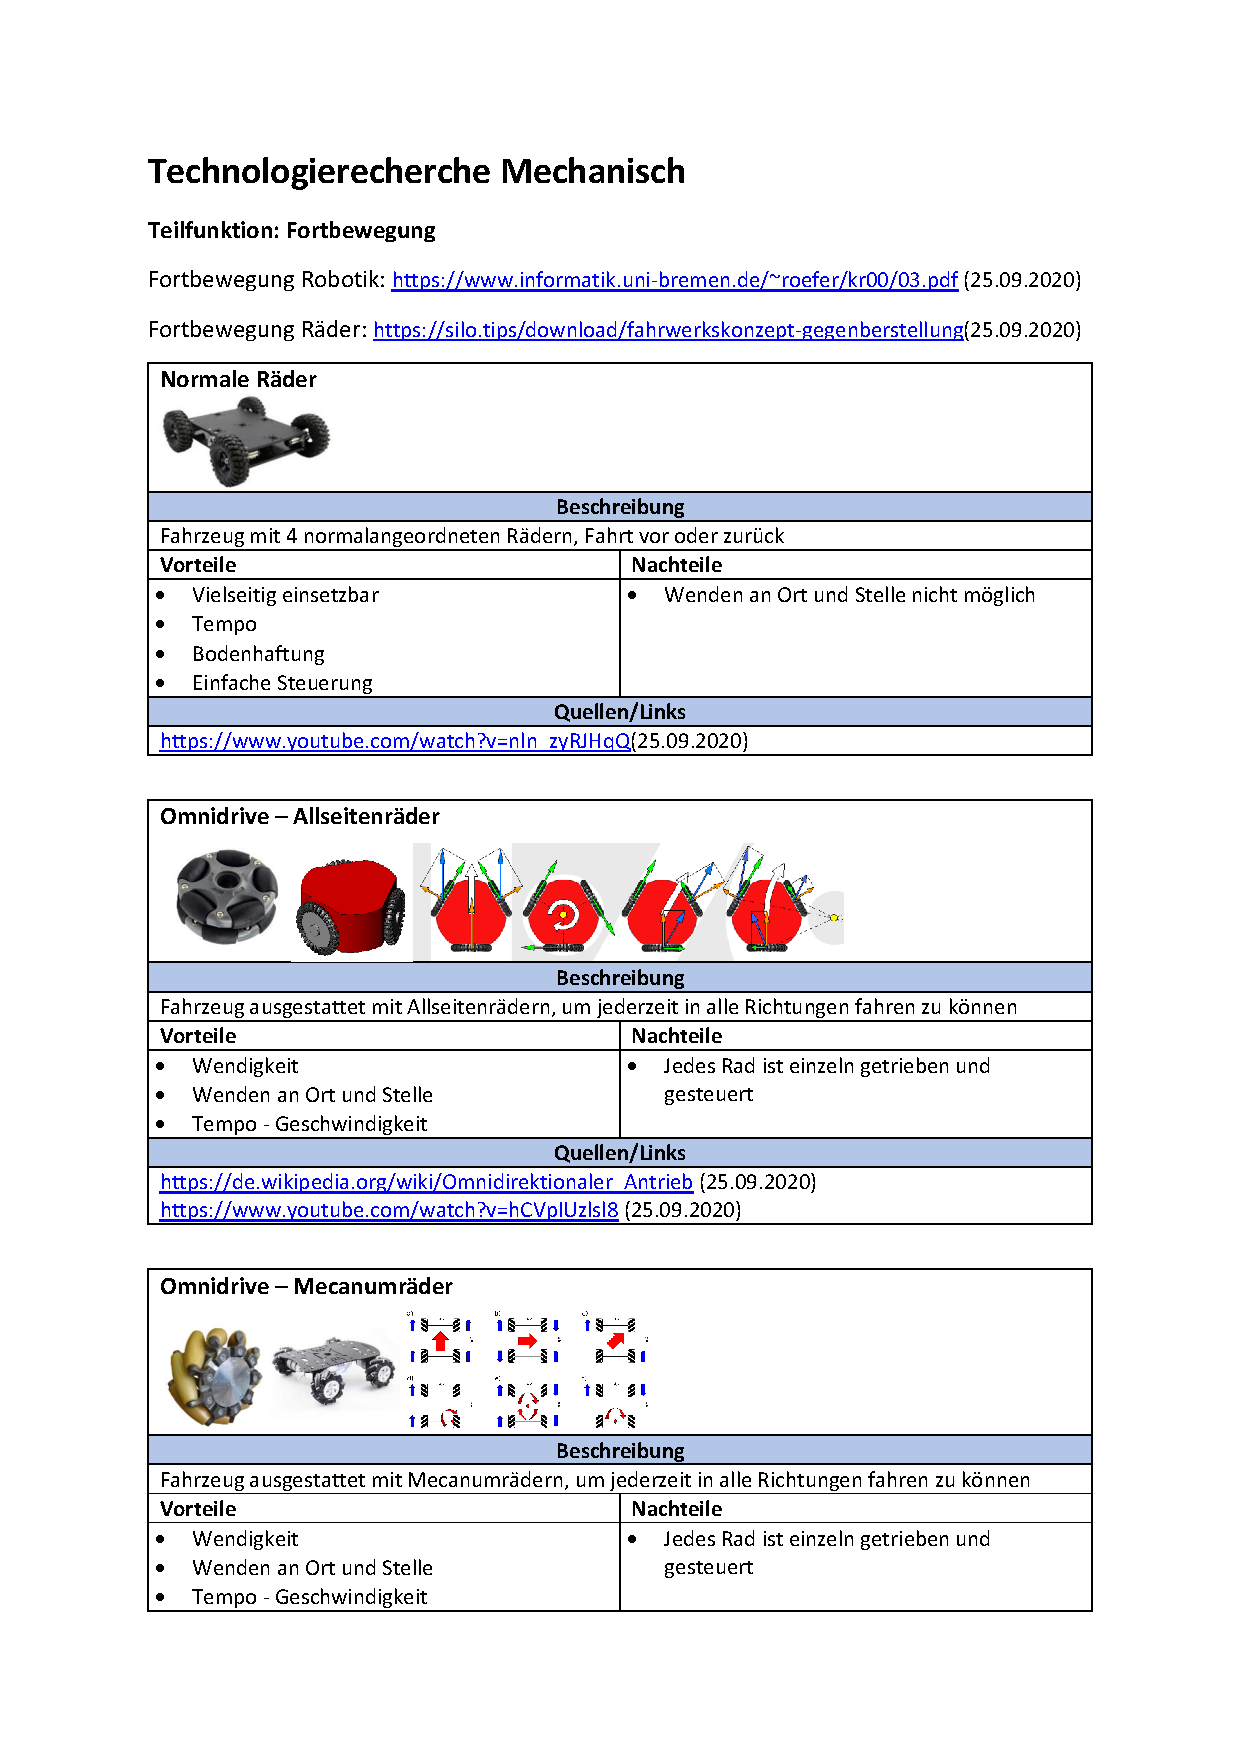
\includepdf[
  pages={1-},
  scale=1,
  pagecommand={\pagestyle{fancy}}
]{assets/Technologierecherche M.pdf}

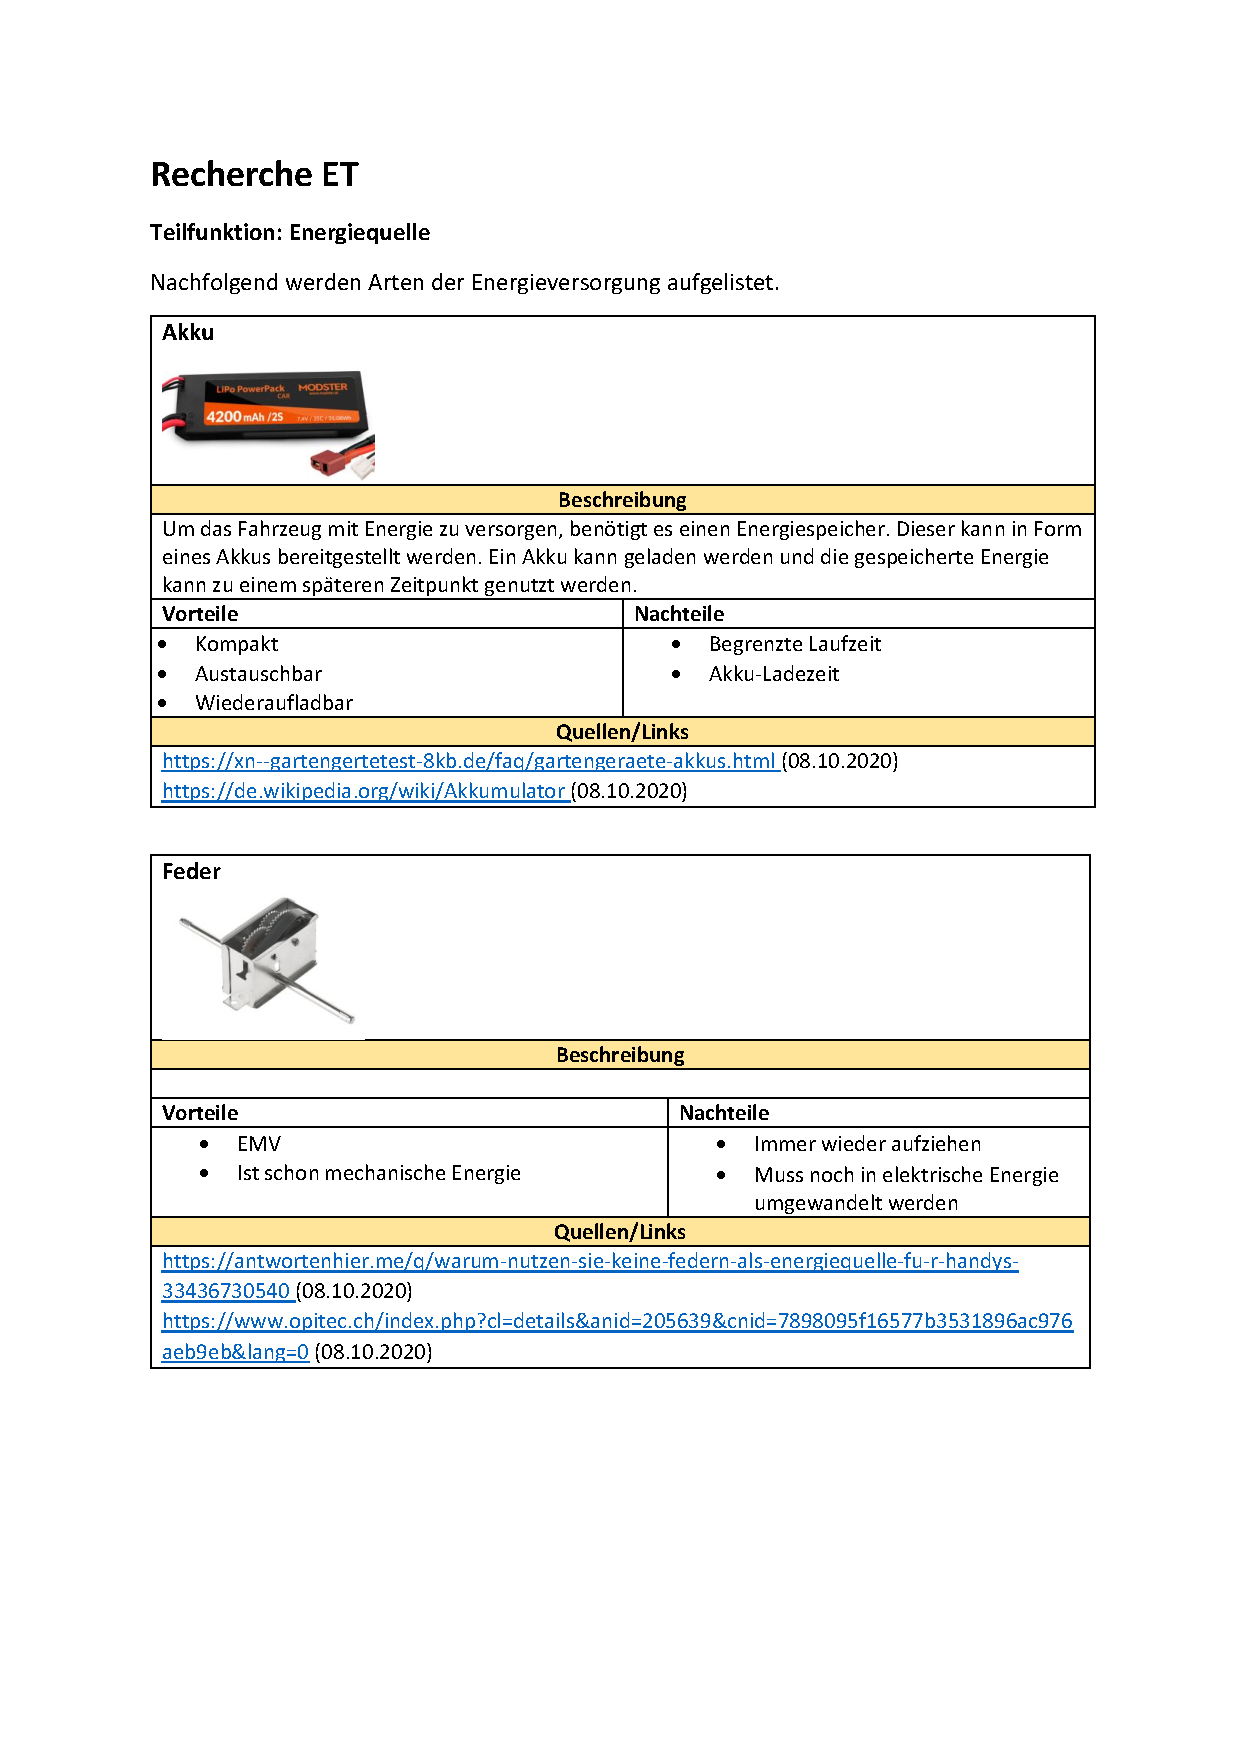
\includepdf[
  pages={1-},
  scale=1,
  pagecommand={\pagestyle{fancy}}
]{assets/Technologierecherche ET.pdf}

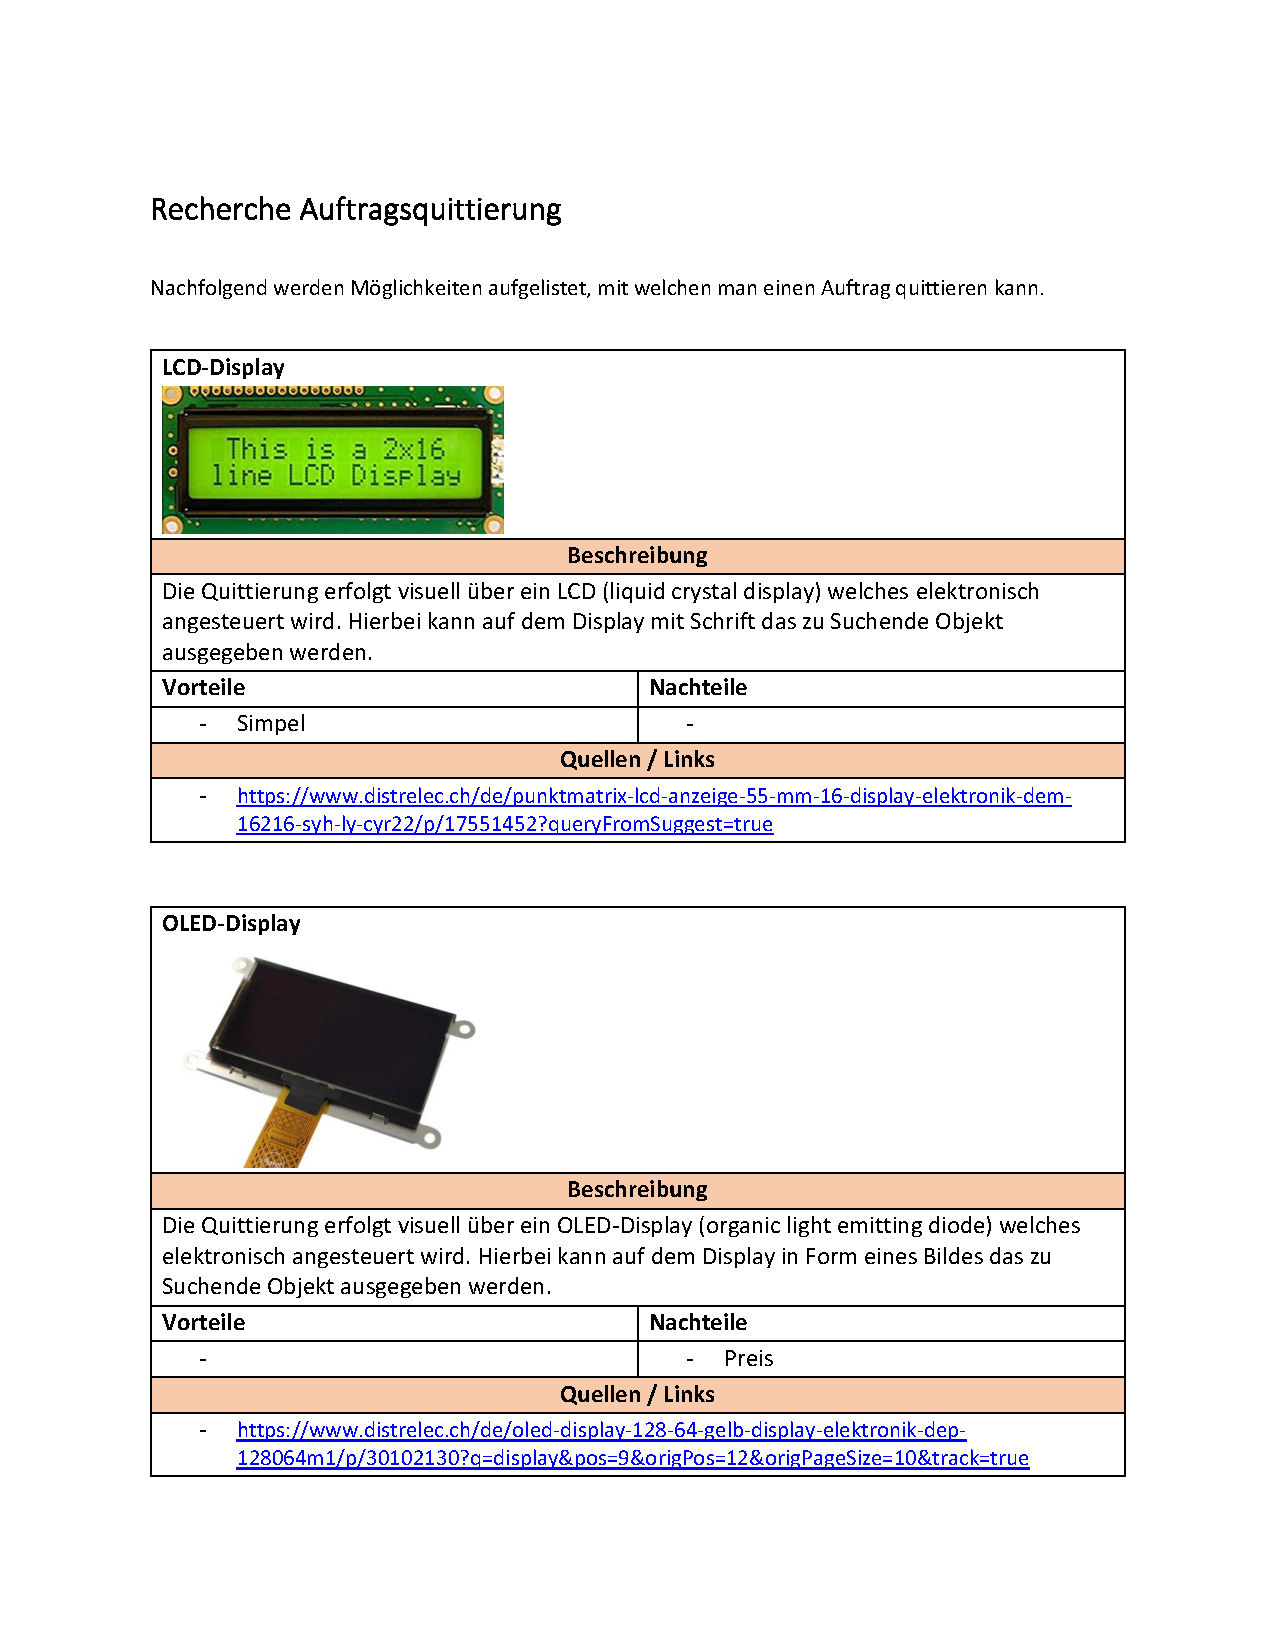
\includepdf[
  pages={1-},
  scale=1,
  pagecommand={\pagestyle{fancy}}
]{assets/Recherche Auftragsquittierung.pdf}

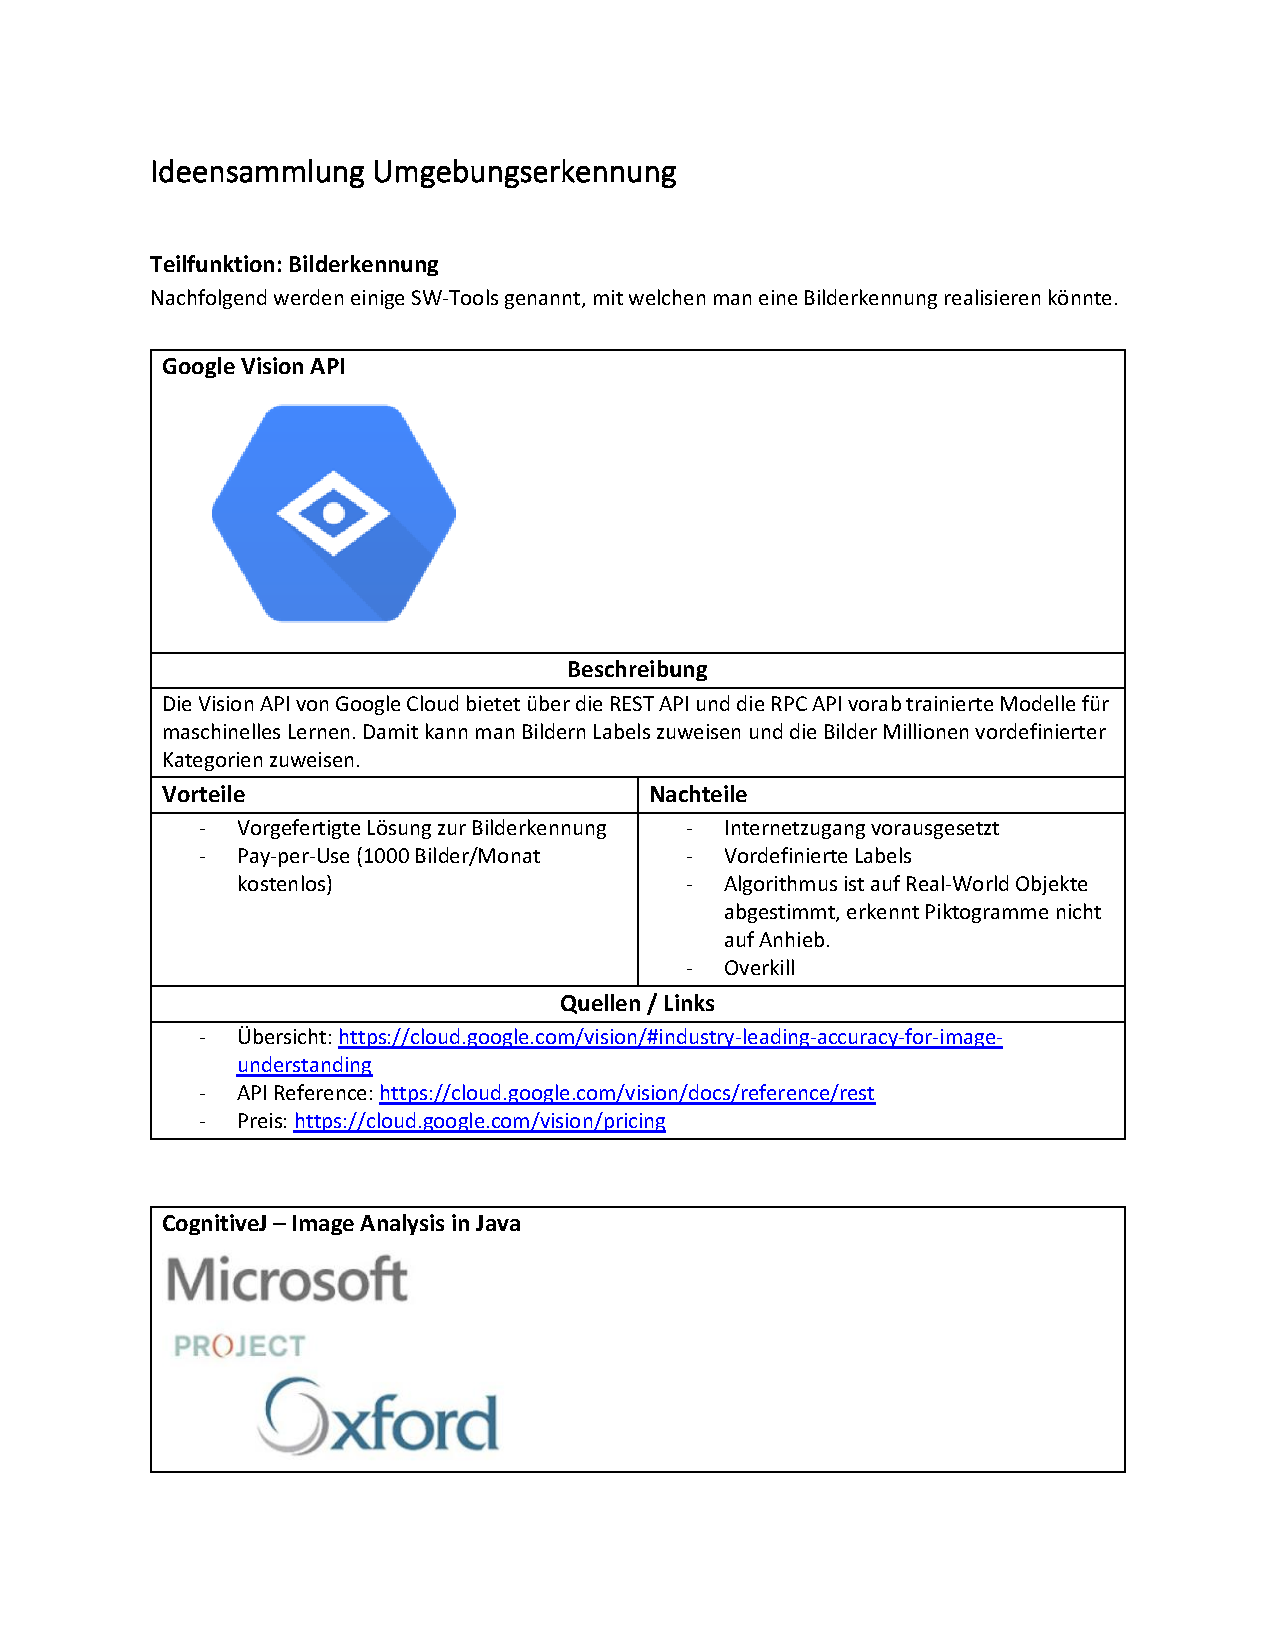
\includepdf[
  pages={1-},
  scale=1,
  pagecommand={\pagestyle{fancy}}
]{assets/Recherche Umgebungserkennung.pdf}

